\documentclass{scrreprt}
\usepackage[english]{babel}
\usepackage[T1]{fontenc}
\usepackage{lmodern}
\usepackage{blindtext}
\usepackage[utf8]{inputenc}
\usepackage{siunitx} %For unit handling%
\renewcommand{\familydefault}{\sfdefault}
\newcommand{\unit}[1]{\ensuremath{\, \mathrm{#1}}}
\usepackage{amssymb, amsmath, cancel, ulem, graphicx, float, tabularx, multirow, bm}
\usepackage{amsmath}
\usepackage{caption}
\usepackage{subcaption}
\usepackage{mathtools}
\usepackage{tikz}
\usepackage{commath}
\usepackage{nameref}
\newcommand*\circled[1]{\tikz[baseline=(char.base)]{
            \node[shape=circle,draw,inner sep=1pt] (char) {#1};}}
\renewcommand{\phi}{\varphi}


\setcounter{secnumdepth}{5}
\setcounter{tocdepth}{5}

\author{Urs Gerber\\09-921-156 \and Gian-Luca Mateo\\11-113-545}
\date{16th of May 2013}

\title{e/m}
\subtitle{Practical course report}

\begin{document}

\maketitle

\tableofcontents
\newpage

\chapter{Experiment: e/m}

\section{Introduction}

\subsection{Goal of the experiment}
 
\subsection{Theory}

\begin{equation}
F_Z = \frac{m v^2}{r}
\end{equation}

\begin{equation}
F_L = e v B
\end{equation}

\begin{equation}
F_Z \stackrel{!}{=} F_L \Longrightarrow \frac{e}{m} = \frac{v}{r B}
\end{equation}

\begin{equation}
e U = \frac{1}{2} m v^2 \Longrightarrow v = \sqrt{\frac{2 e U}{m}}
\end{equation}

\begin{equation}
\Longrightarrow \frac{e}{m} = \frac{2 U}{r^2 B^2}
\end{equation}

\begin{equation}
B_z (0) = \left( \frac{4}{5}\right)^{\frac{3}{2}} \frac{\mu_0 N I}{R}
\end{equation}

\subsubsection{Error analysis}

\begin{equation}
s_r^2 = \frac{r^2\cdot s_l^2}{(L-l)^4} + \frac{r^2\cdot s_L^2}{(L-l)^4}
\end{equation}

\begin{equation}
s_{e/m} = 4 \frac{s_r U}{B^2 r^3}
\end{equation}

\section{Experiment setup and execution}

\subsection{Used materials}
The materials used in this experiment are the following:
\begin{itemize}
\item A Teltron tube with 2 Helmholtz coils
\item An optical bench
\item A small mask and a circle template, both mountable to the bench
\item 3 power supply units
\end{itemize}

\subsection{Assembly and Execution}
For this experiment, the Teltron tube and the Helmholtz coils are connected to the power supplies and powered on. As soon as the electron beam is visible, the amperage of the Helmholtz coils is increased up to the point where the electron beam marks a circular trail. Using the mask and the template, the radius of the circle is measured. This procedure is then repeated for some acceleration voltages and different coil amperages.

\section{Measurements}
All measurements were taken at a heating voltage of $U_h = (8 \pm 0.01) \unit{V}$. The focussing voltage $U_f$ was varied between $0 \unit{V}$ and $30 \unit{V}$.

\begin{figure}[H]
	\centering
  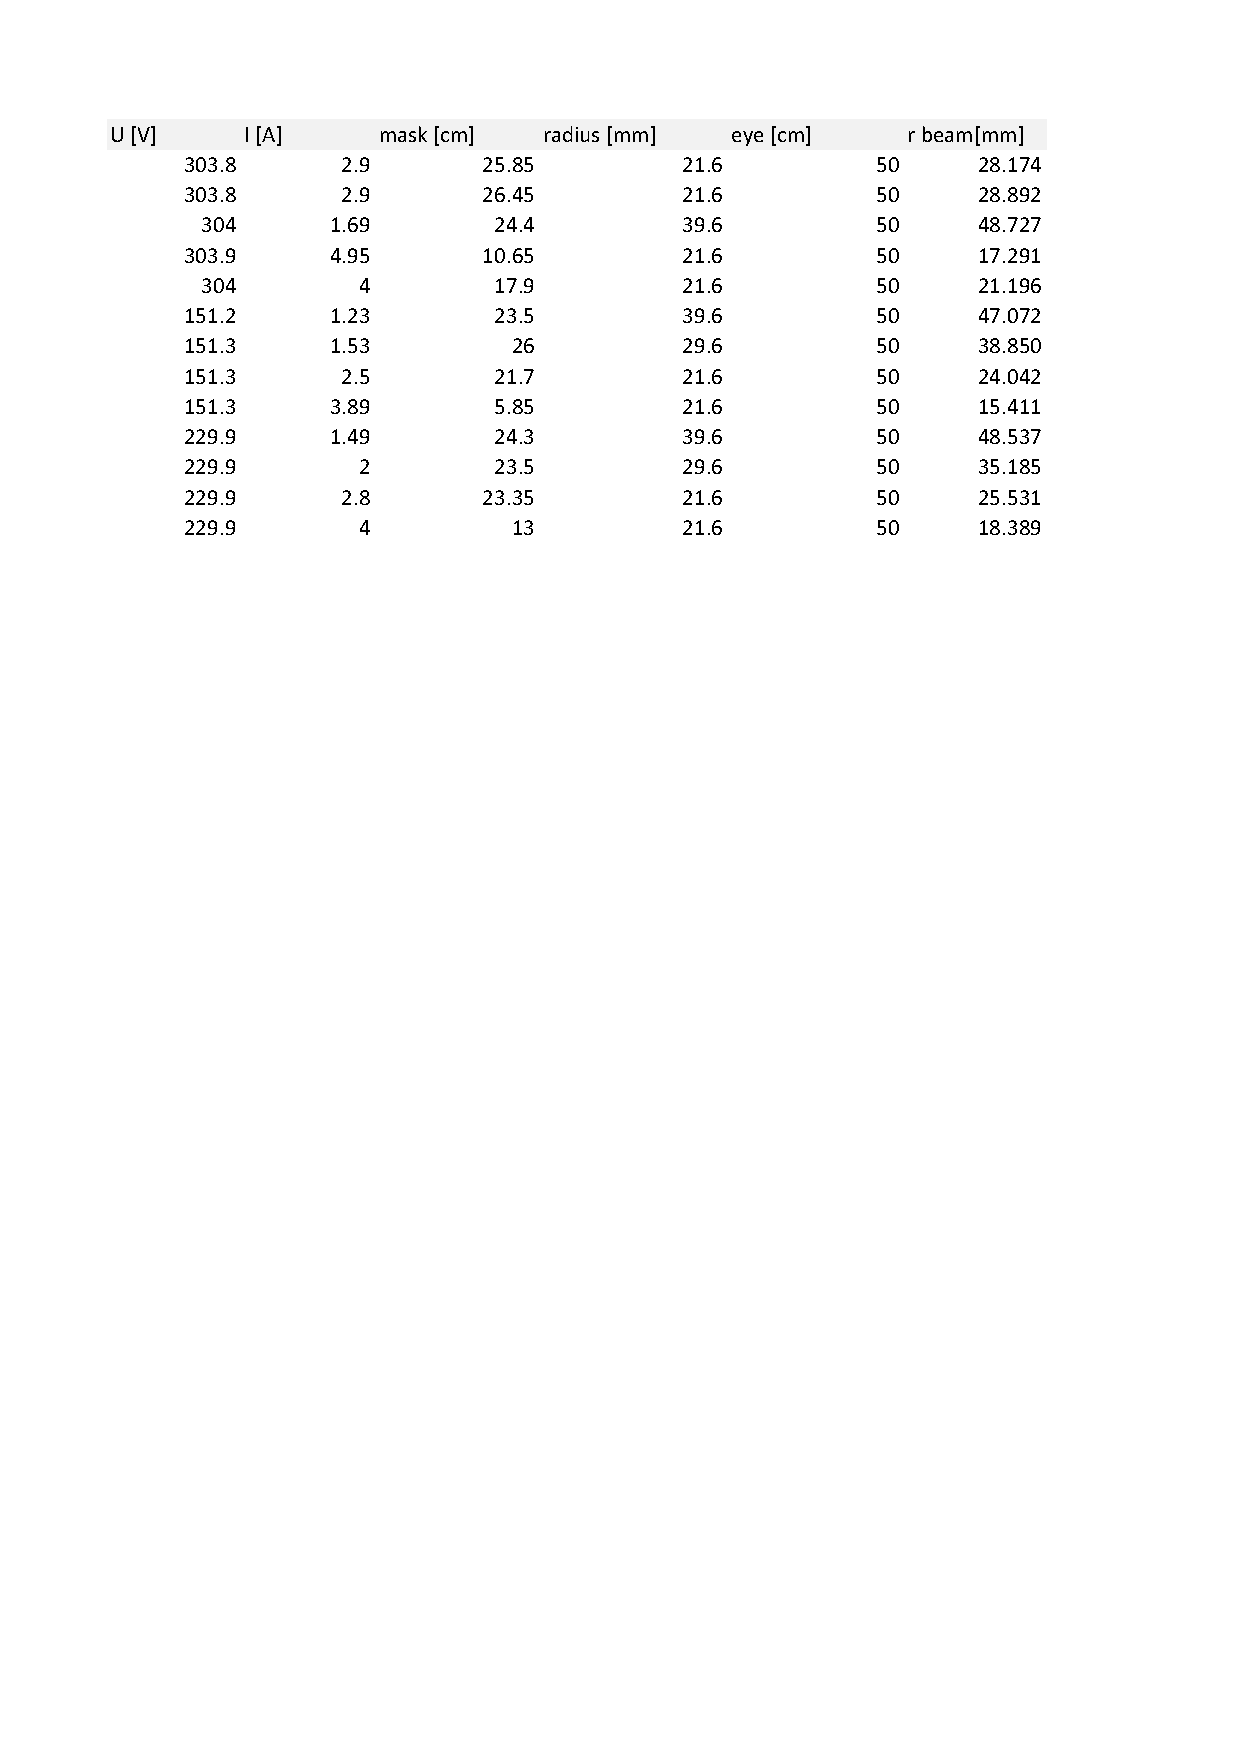
\includegraphics[width=0.9\textwidth]{diag/measurements.pdf}
	\caption{Measured radii $r$ for different values of $U$ and $I$}
	\label{fig:measurements}
\end{figure}

\section{Analysis and Discussion}

Using all our measurements and error analysis formulae we can deduct the following values:

\begin{table}[H]
\center
\begin{tabular}{|c|c|c|c|c|c|}
\hline
$U$ [$\unit{V}$] & $I$ [$\unit{A}$] & $r$ [$\unit{mm}$] & $r_{\text{theo}}$[$\unit{mm}$] & $e/m \cdot 10^{11}$ & rel. $\Delta$\\ \hline\hline
$303.8$ & $2.90$ & $28.174 \pm 1.126$ & $27.266$ & $1.647 \pm 0.132$ & $-6.77 \%$\\
$303.8$ & $2.90$ & $28.892 \pm 1.185$ & $27.266$ & $1.566 \pm 0.128$ & $-12.28 \%$\\
$304.0$ & $1.69$ & $48.727 \pm 1.828$ & $46.804$ & $1.623 \pm 0.122$ & $-8.39 \%$\\
$303.9$ & $4.95$ & $17.291 \pm 0.424$ & $15.977$ & $1.502 \pm 0.074$ & $-17.13 \%$\\
$304.0$ & $4.00$ & $21.196 \pm 0.638$ & $19.775$ & $1.531 \pm 0.092$ & $-14.90 \%$\\
$151.2$ & $1.23$ & $47.072 \pm 1.715$ & $45.352$ & $1.633 \pm 0.119$ & $-7.73 \%$\\
$151.3$ & $1.53$ & $38.850 \pm 1.563$ & $36.472$ & $1.550 \pm 0.125$ & $-13.47 \%$\\
$151.3$ & $2.50$ & $24.042 \pm 0.820$ & $22.321$ & $1.516 \pm 0.103$ & $-16.02 \%$\\
$151.3$ & $3.89$ & $15.411 \pm 0.337$ & $14.345$ & $1.524 \pm 0.067$ & $-15.42 \%$\\
$229.9$ & $1.49$ & $48.537 \pm 1.823$ & $46.165$ & $1.591 \pm 0.120$ & $-10.54 \%$\\
$229.9$ & $2.00$ & $35.185 \pm 1.282$ & $34.393$ & $1.681 \pm 0.122$ & $-4.66 \%$\\
$229.9$ & $2.80$ & $25.531 \pm 0.925$ & $24.566$ & $1.628 \pm 0.118$ & $-8.01 \%$\\
$229.9$ & $4.00$ & $18.389 \pm 0.489$ & $17.196$ & $1.538 \pm 0.080$ & $-14.35 \%$\\
\hline
\end{tabular}
\end{table}

In order to estimate the error of $l$ we measured this quantity twice at the same parameters and we found $s_l = 3 \unit{mm}$

\begin{equation}
e/m = \left( 1.579 \pm 0.0161 \right)\cdot 10^{11} \unit{\frac{coul}{kg}}
\end{equation}

\subsection{Sources of error}
\label{sec:error}
Looking for sources of error, we found very few. Both the amperage and the voltage were measured accurately and the measurements showed no reason to doubt that. Errors in the calculation of the strength of the magnetic field can be ruled out, as our documents stated a relative error obtained by using the formulae used being less than $2\%$ \cite[p. 174]{physcript13}. 
The only relevant source of error lies in the measurement of the diameter of the electron beam. We always tried to see the whole beam through the mask, which probably accounts for too large radii. 
\begin{figure}[H]
	\centering
  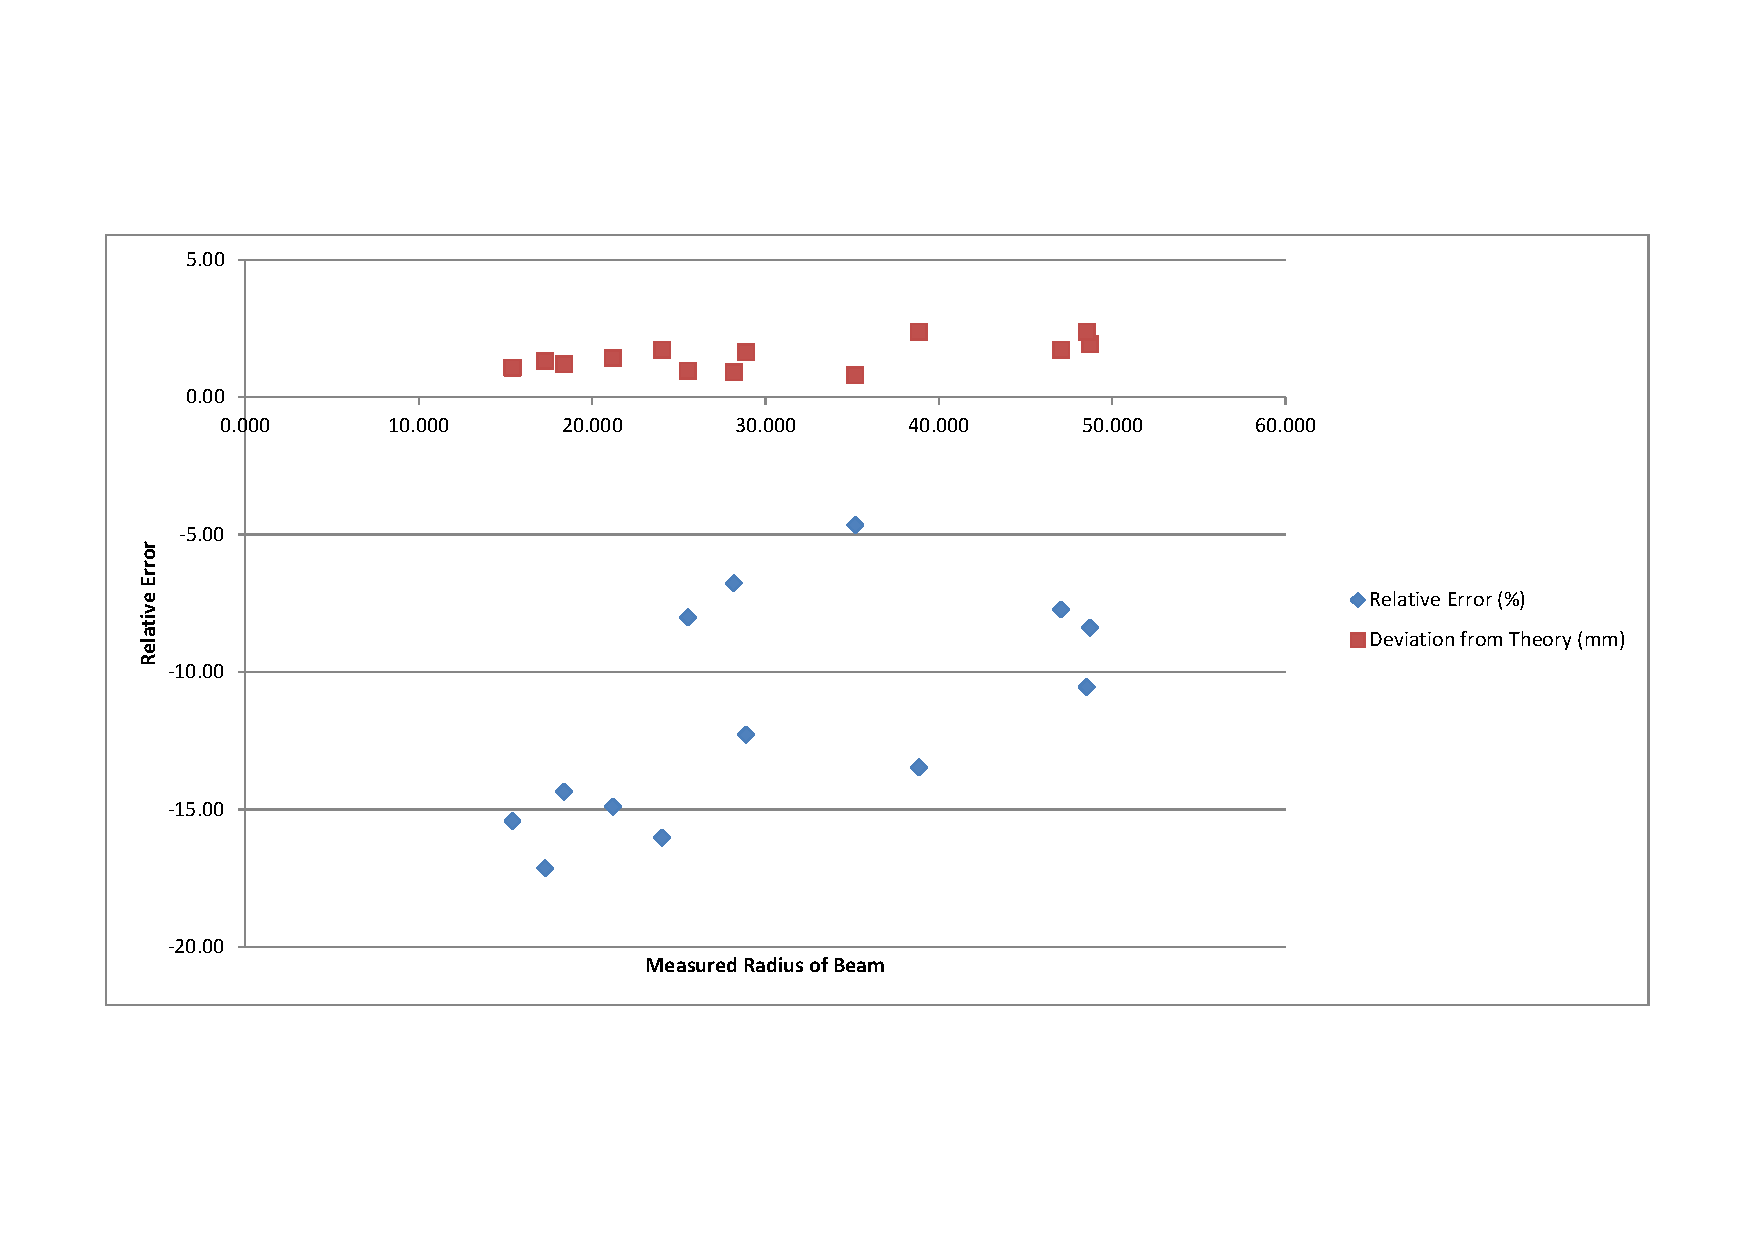
\includegraphics[width=0.9\textwidth]{diag/errors.pdf}
	\caption{Deviation from Theoretical Values for Radii and Relative Error}
	\label{fig:error}
\end{figure}

Looking at \ref{fig:error}, that point can be further supported. The errors for the radii do not see the same order of dependance from the radii as the relative error.

\section{Conclusion}

\begin{thebibliography}{9}

\bibitem{physcript13}
  Peter Wurz,
  \emph{Anleitung zum Physikpraktikum}
  FS2013

\end{thebibliography}

\end{document}
